\newcommand\withLogo[2]{\raisebox{-.25\height}{\includegraphics[keepaspectratio=true,height=27pt]{#1}}~~#2}
\newcommand\no{\Large $\times$}
\newcommand\yes{\Large $\checkmark$}

\section{Introduction}
\begin{frame}[plain]


\renewcommand{\arraystretch}{2.5}
\begin{tabular}{l|l|c|c}
\textbf{\hfil\small Blockchain\hfil} & \textbf{\hfil\small Model\hfil} & \textbf{\small Turing-complete} & \textbf{\small Deterministic} \\
\hline
\withLogo{bitcoin}{Bitcoin} & UTXO & \no & \yes \\
\hline
\hspace{3pt}\withLogo{ethereum}{\hspace{3pt}Ethereum} & Accounts & \yes & \no \\
\hline
\withLogo{ada}{Cardano (IOHK)} & UTXO$^{++}$ & \yes & \yes \\
\end{tabular}

\end{frame}

\begin{frame}{Methodology}
\begin{itemize}
\item Focus on validating the relevant meta-theory
  \begin{itemize}
  \item In contrast to validating individual contracts
  \end{itemize}
\item Fully mechanized approach, utilizing Agda's rich type system
\item Fits well with IOHK's research-oriented approach
\end{itemize}

\begin{tikzpicture}
  [basic box/.style = {
     draw,
     shape = rectangle,
     align = center,
     minimum width=2cm,
     minimum height=1.2cm,
     rounded corners},
   to/.style = {
     ->,
     >=stealth',
     semithick
  },
  every matrix/.style={column sep=.8cm, ampersand replacement=\&},
  font=\small
  ]
  \matrix{
     \node[basic box,draw=mLightBrown] (a) {pure\\ research};
  \& \node[basic box,draw=mLightBrown] (b) {mechanized\\ models};
  \& \node[basic box] (c) {reference\\ implementations};
  \& \node[basic box] (d) {production\\ code}; \\
  };

  \path
  (a) edge[to, mLightBrown] (b)
  (b) edge[to] (c)
  (c) edge[to] (d)
  ;
\end{tikzpicture}
\end{frame}

\begin{frame}[label=contributions]{Contributions}

\begin{itemize}
\setlength\itemsep{.25cm}

\item \textbf{Detailed description of the Extended UTXO model (EUTXO)}
\begin{center}
\scalebox{.7}{
  \begin{tikzpicture}
    \eutxo
  \end{tikzpicture}
}
\end{center}

\item \textbf{Formalization in} \raisebox{-.5\height}{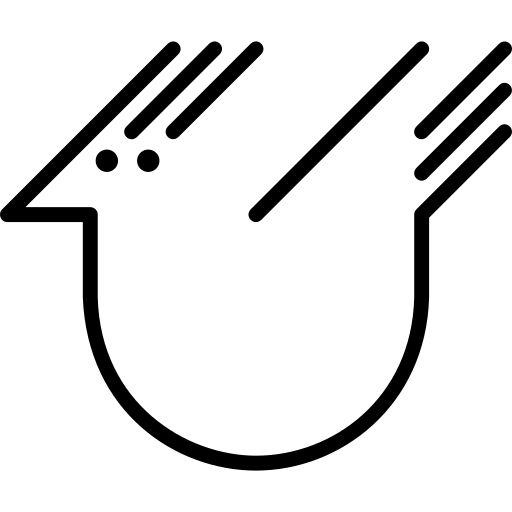
\includegraphics[height=.18\textheight]{agda}}\\

\item \textbf{Proof of bisimulation with a specific form of state machines}\\
\begin{center}
\scalebox{.6}{
  \begin{tikzpicture}
    \multisig
  \end{tikzpicture}
}
\end{center}

\end{itemize}

\end{frame}
